%% ID: acceleration_string
%% TITLE: Acceleration on a String
%% TYPE: question
%% QUESTIONTYPE: numeric
%% CONCEPTS: energy, momentum
%% VIDEOS: 
%% LEVEL: 3
%% TOPIC: mechanics/dymanics
%% ORDER: 5

\begin{problem}[AO1984PIQ1a]
{A particle Q of mass 2 kg is resting on a frictionless surface. It is attached to one end of a piece of elastic string, with the other end of the elastic being attached to a fixed point. Q is then pulled back and released from rest with the elastic extended 0.5 m beyond its natural length. 

After the particle has been accelerated, the string becomes slack. Rather than being let to continue in some kind of oscillatory motion, the string is cut when it first becomes slack. It is travelling at a speed of 4 ms$^{-1}$ when this occurs.

Assuming no losses to friction or other dissipative forces:
\begin{enumerate}
	\item Calculate the energy stored in the elastic, and the maximum tension in the elastic during the process.
\end{enumerate}
Q then makes an elastic collision with a stationary body P and rebounds back along the same track at 3.0 ms$^{-1}$. 
\begin{enumerate}[resume]
	\item Calculate the mass of P, and its velocity after the collision.
	\item If Q had instead been accelerated from rest by a small motor giving a power of 40 W, how long would it have taken to reach a speed of 4.0 ms$^{-1}$?
\end{enumerate}
\vspace{-0.4cm}
}
{\textit{Adapted with permission from UCLES, AO Level Physics, November 1984, Paper 1, Question 1.}}
{\begin{enumerate}
	\item If there are no losses to friction or other forces, then the energy stored in the elastic must go completely into the kinetic energy of P. Thus the energy stored in the elastic, $E$, is given by:
\begin{align*} E = \frac{1}{2}mv^{2} = \frac{1}{2}(2)(4)^{2} \textrm{ J} = 16 \textrm{ J} \end{align*}

In order to work out the maximum tension; we need to relate the tension in the elastic to the extension: the force required to stretch the elastic is $\vtr{F} = k\vtr{x}$ where $k$ is commonly called the spring constant, and so the tension, which is equal in magnitude but opposite in sign, must be $kx$. The constant $k$ can be found by considering the energy stored $E = \frac{1}{2}kx^{2}$ and we know both $E$ and $x$:
\begin{equation*} k = \frac{E}{x^{2}} = \frac{16}{(0.5)^{2}} \textrm{ N m}^{-1} = 128 \textrm{ N m}^{-1} \end{equation*}
and so the tension, which is maximum at the maximum extension, is:
\begin{equation*} T\s{max} = kx = (128)(0.5) \textrm{ N} = 64 \textrm{ N} \end{equation*}
	\item To find the mass and velocity of P after the collision, it is first easiest to find the momentum and kinetic energy. The collision is elastic, and so both momentum and kinetic energy are conserved. A diagram, as in Figure \ref{fig:Dynamics_PQ_mass}, is useful.
	
\begin{figure}[h]
	\centering
	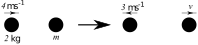
\includegraphics[width=0.6\textwidth]{Dynamics_PQ_mass}
	\caption{}
	\label{fig:Dynamics_PQ_mass}
\end{figure}

Conserving momentum, taking care of the directions of the velocities, and labelling the momentum of P as $p$gives:
\begin{align*} (2)(4) &= (2)(-3) + p\s{P}  \\ p &= 14 \textrm{ kg ms}^{-1}\end{align*}
and conservation of energy implies that:
\begin{align*} \frac{1}{2}(2)(4)^{2} &= \frac{1}{2}(2)(3)^{2} + E\s{P}  \\ E\s{P} &= 7 \textrm{ J} \end{align*}

Now we can use the fact that $p = mv$ and $E\s{P} = \frac{1}{2}mv^{2}$ as simultaneous equations to solve for $m$ and $v$.

\begin{align*} p = mv = 14 &&  2E\s{P} = mv^{2} = 14 \\ \intertext{so since $v^{2} = v$, it follows:} v = 1 \textrm{ ms}^{-1} && m = 14 \textrm{ kg} \end{align*}

	\item The energy input from the motor would have to equal the kinetic energy gained by Q (assuming perfect efficiency), so simply equate Energy = Power $\times$ Time with $\frac{1}{2}mv^{2}$:

\begin{align*} Pt &= \frac{1}{2}mv^{2} \\ 40t &= 16 \\ t&=0.4\textrm{ s} \end{align*}

\end{enumerate}
}
\end{problem}